%!TEX root = ../Main.tex
\section{Benchmarks}
\label{s:Benchmarks}

We are currently using Icicle in production, over medium-sized datasets that fit on a single disk.
Initial results have been very promising, and we are currently working towards a distributed implementation for larger datasets.

One evaluation we performed was replacing a hand-written R script which had been running in production.
This R script works over around three hundred gigabytes of PSV data.
It computes twelve queries over each of the thirty-one input tables, computing 372 queries in total.

The R script for this takes around fifteen hours to run and is 3,566 lines, 2,311 of which are code.
In contrast, our Icicle queries take eleven minutes to run, and the dictionary describing the queries is 191 lines of code.

It is also important to note that, as a very constrained streaming language, memory usage of Icicle queries is more or less constant in the input size, and runtime is linear.
This is very important, as new data is received regularly and the input size grows.
This does not appear to be the case with the R script, which continually requires larger computers with more memory, in order to finish in a reasonable time.
One of the benefits of Icicle is allowing data scientists to focus on queries, without having to worry about performance.

\begin{figure}

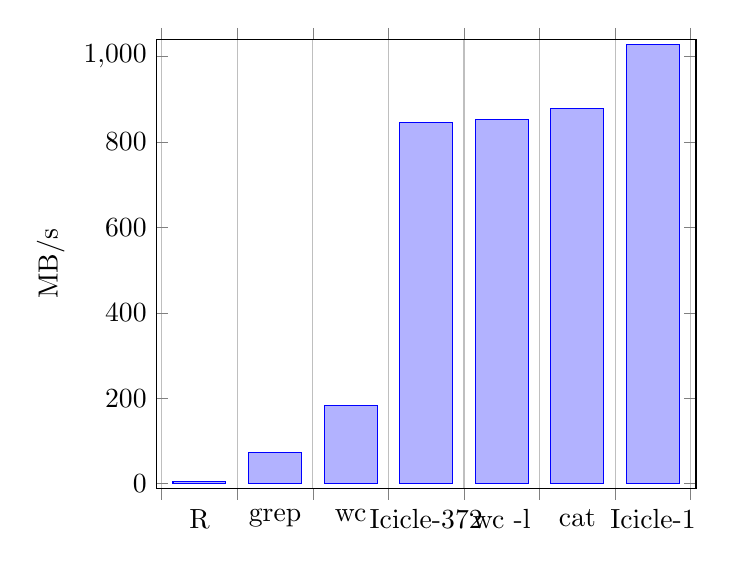
\begin{tikzpicture}
\begin{axis}[
	x tick label style={/pgf/number format/1000 sep=},
	ylabel=MB/s,
	enlargelimits=0.01,
	legend style={at={(0.5,-0.1)},anchor=north,legend columns=-1},
	ybar interval=0.7,
  symbolic x coords={R, grep, wc, Icicle-372, wc -l, cat, Icicle-1, end}
]
\addplot coordinates {(R,6.0) (grep,74) (wc,182.6) (Icicle-372,846) (wc -l,852) (cat,878) (Icicle-1,1029) (end,0) };

% \legend{MB/s}

\end{axis}
\end{tikzpicture}

\caption{Throughput comparisons of Icicle against existing R code and standard unix utilities}
\label{fig:bench:other}
\end{figure}


\begin{figure}

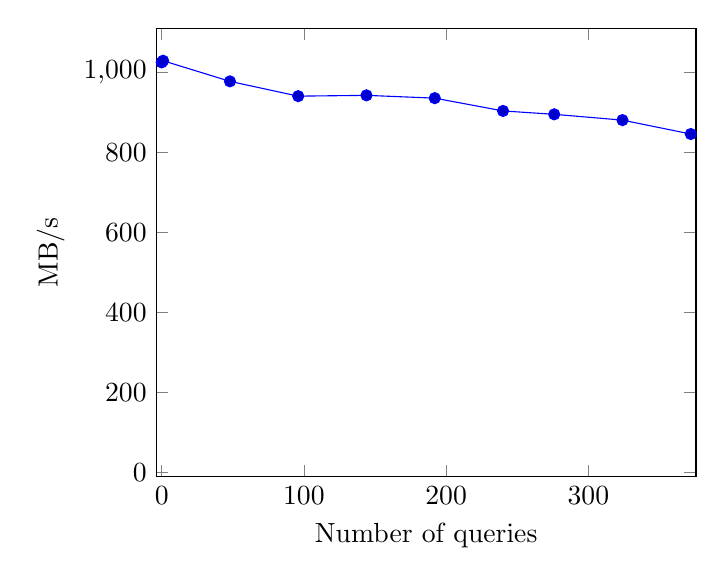
\begin{tikzpicture}
\begin{axis}[
	x tick label style={/pgf/number format/1000 sep=},
	ylabel=MB/s,
  ymin=0, ymax=1100,
%  xmax=372,
  xlabel=Number of queries,
	enlargelimits=0.01,
	legend style={at={(0.5,-0.1)},anchor=north,legend columns=-1},
%	ybar interval=0.7,
]
\addplot coordinates {(0,1025.5) (1,1029.6) (48,978) (96,941) (144,943) (192,936) (240,904) (276,895.5) (324,881) (372,846.2) };

% \legend{MB/s}

\end{axis}
\end{tikzpicture}


\caption{Decrease in throughput as queries are added}
\label{fig:bench:queries}
\end{figure}


The table in figure~\ref{fig:bench:other} shows the throughput in megabytes per second.
We compared the throughput of several programs over the same 360GB dataset:
\begin{itemize}
\item our original R implementation (R);
\item Icicle with equivalent queries (Icicle-372);
\item Icicle with a single query computing the mean (Icicle-1);
\item finding empty lines with @grep "^$"@;
\item counting characters, words and lines with @wc@;
\item counting only lines with @wc -l@; and
\item the sequential read speed of the disk (@disk@).
\end{itemize}
All of the unix utilities were run with the collation set to @LANG=C@ for maximum performance.

It is heartening to see that both Icicle runs outperform @R@, @grep@ and @wc@, while the single query even outperforms @wc -l@.

